% 敏感性分析
\section{敏感性分析}
\label{sec:sens}

围绕模型的关键参数做系统性扰动，检验结论的结构稳定性。各项数值均来自对
最新求解产物的重算。

\subsection{返航安全余量比例的敏感性}

安全余量比例 $\rho$ 直接决定单架次可用能量，进而决定最大安全载荷、架次数与
总能耗。扫描结果如表 \ref{tab:rho} 所示，图 \ref{fig:rho} 给出架次与能耗的
变化曲线。$\rho$ 在 0.1 至 0.2 区间内架次与能耗不变，均为 18 架次、59.02\,kWh，
说明 20\% 的安全余量下效率尚有富余；$\rho$ 增至 0.25、0.30、0.35 时远区
C 型架次被逐步拆分，架次增至 19、20、25，能耗升至 60.96、67.10、77.63\,kWh，
安全换效率的代价加速显现；$\rho$ 由 0.35 增至 0.40 时架次数不变而能耗由
77.63 降至 74.62\,kWh，源于机型结构切换，即部分 C 型远区任务改由更经济的
组合完成。该曲线为应急指挥在安全与效率之间的权衡提供了直接依据。

\begin{table}[htbp]
\centering
\caption{返航安全余量比例对问题一方案的影响}
\label{tab:rho}
\begin{tabular}{lccccccc}
\toprule
$\rho$ & 0.10 & 0.15 & \textbf{0.20} & 0.25 & 0.30 & 0.35 & 0.40 \\
\midrule
架次数 & 18 & 18 & \textbf{18} & 19 & 20 & 25 & 25 \\
总能耗(kWh) & 59.02 & 59.02 & \textbf{59.02} & 60.96 & 67.10 & 77.63 & 74.62 \\
\bottomrule
\end{tabular}
\end{table}

\begin{figure}[htbp]
\centering
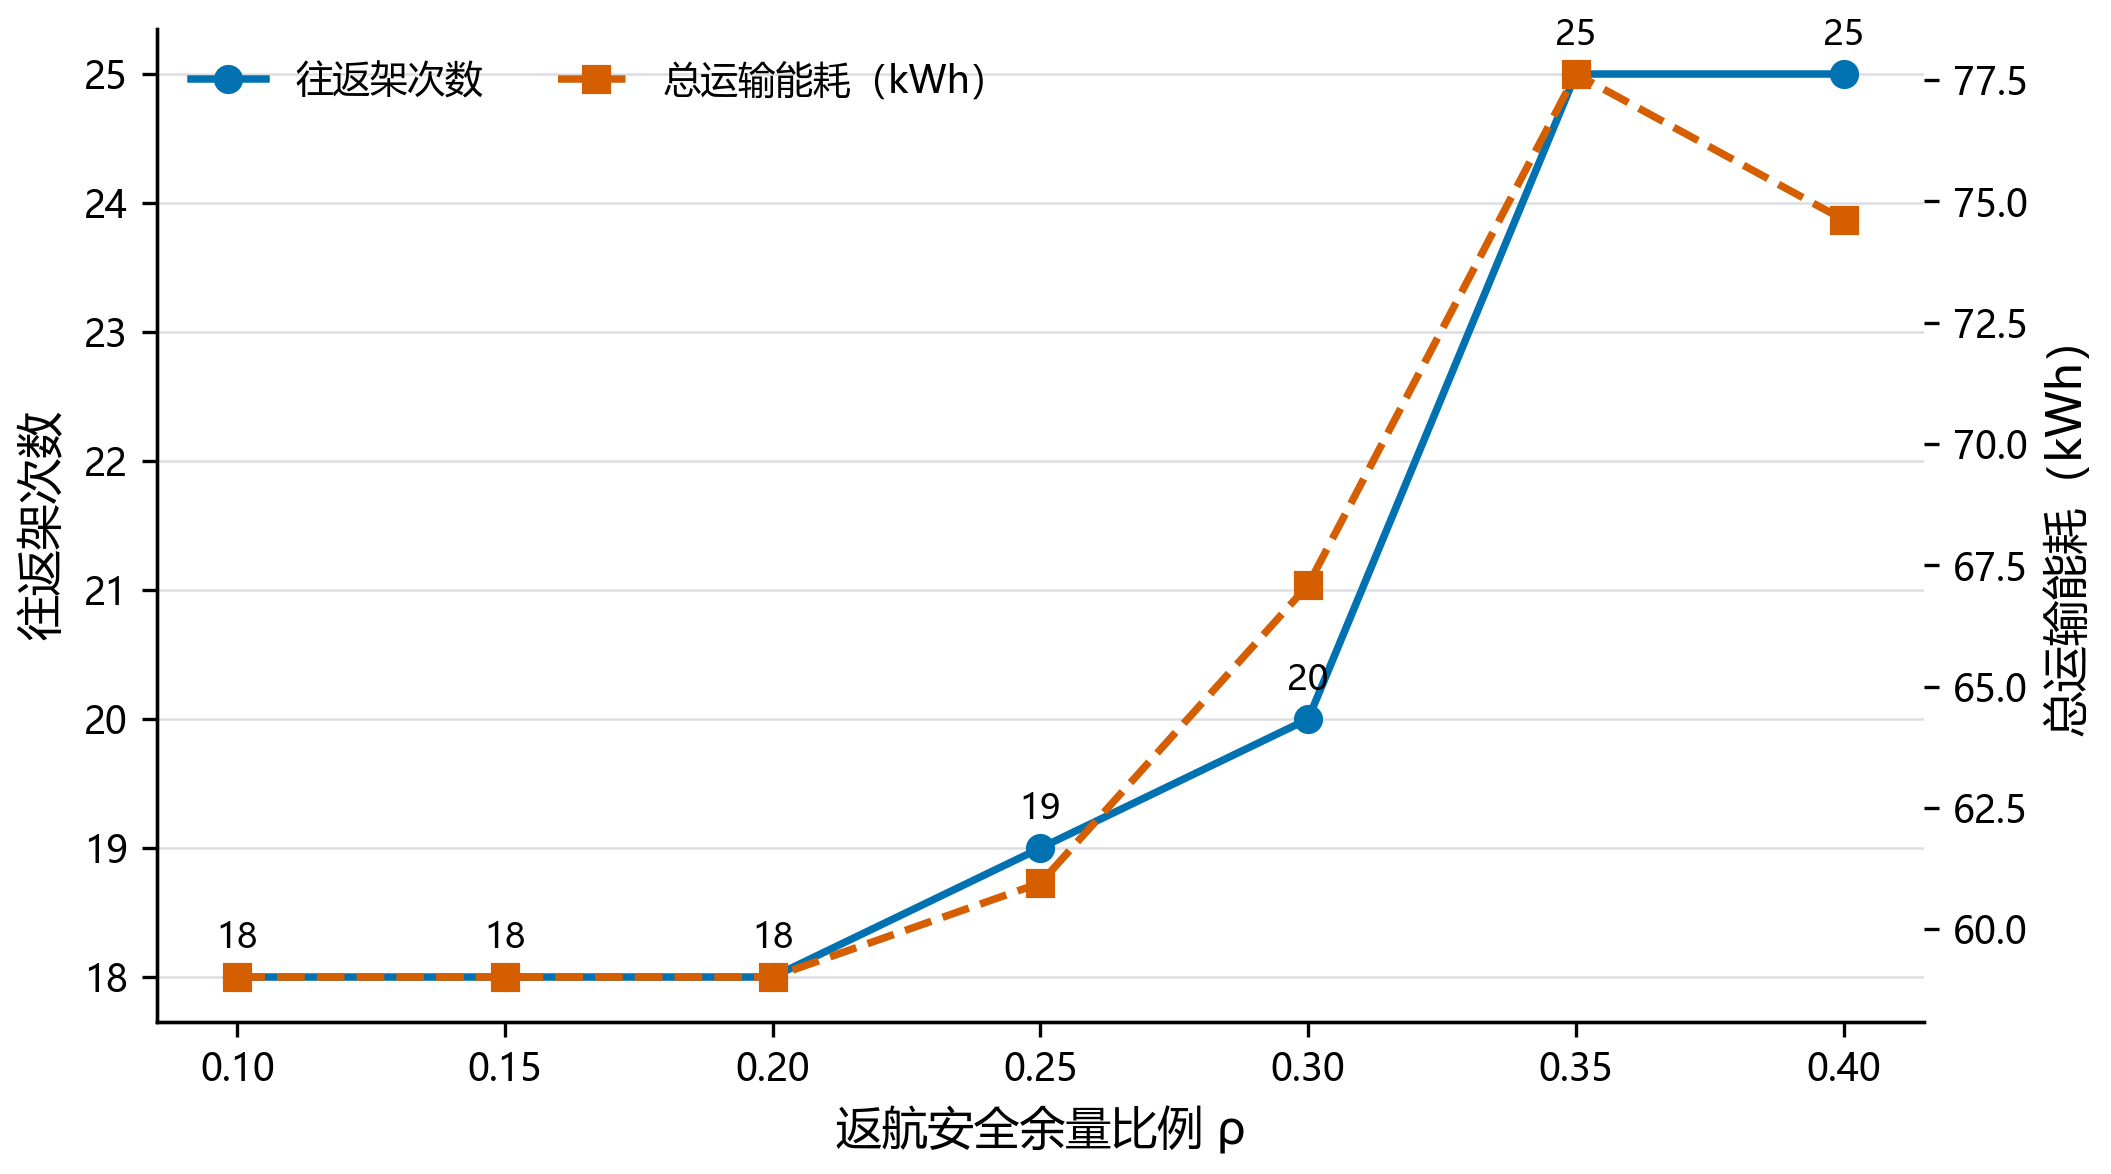
\includegraphics[width=0.74\textwidth]{figures/p1_sensitivity.png}
\caption{返航安全余量比例对架次数与总能耗的影响}
\label{fig:rho}
\end{figure}

\subsection{多目标权重的敏感性}

问题二目标函数含迟到、架次、完工、能耗四项权重。对禁忌搜索进行权重扫描，得到
7661.5\,s/73.73\,kWh、7983.2\,s/72.98\,kWh、8337.0\,s/68.06\,kWh 与
8490.3\,s/65.39\,kWh 四组零迟到方案，见表 \ref{tab:pareto}。不同权重只改变架次拆分粒度与
完工—能耗权衡，不改变重载区由 C 型承担、轻载区由 A/B 型承担的结构结论。

\subsection{中继能源预算的敏感性}

中继单架次服务时长上限由悬停转发功率决定，即 2.56\,kWh 预算除以 1.1\,kW，
约 8378\,s。本文西点连续服务 7083\,s，占上限的 84.5\%，留有约 15.5\%
余量。若未来任务量增长使时段超过上限，可将西点时段拆为两段并
在间隙返场充电，6 组能源组件支持轮换，中继方案结构不变。把悬停转发功率提高
10\%，即由 1.1\,kW 增至 1.21\,kW，上限降至约 7616\,s，仍大于 7083\,s，
方案不受影响。

\subsection{通信链路余量的敏感性}

对全部需中继采样点统计各布设点的接入链路余量，即 116\,dB 减去链路损耗，
结果如表 \ref{tab:margin} 所示，图 \ref{fig:marginhist} 给出三个布设点的余量
分布直方图。西点覆盖 1096 个采样，最紧余量 0.5\,dB，其中有 4 个采样点余量
低于 1\,dB；东点覆盖 484 个采样，最紧余量 1.0\,dB；北点覆盖 211 个采样，
最紧余量 13.4\,dB。若把接收门限提高 1\,dB，即可用余量下压 1\,dB，仅西点的
4 个采样点低于门限，只需对西点布设位置做小幅移位即可恢复全部覆盖；东点与
北点不受影响。布设方案整体对链路参数不敏感，且敏感点集中于个别低空采样，
工程上易于处理。

\begin{figure}[htbp]
\centering
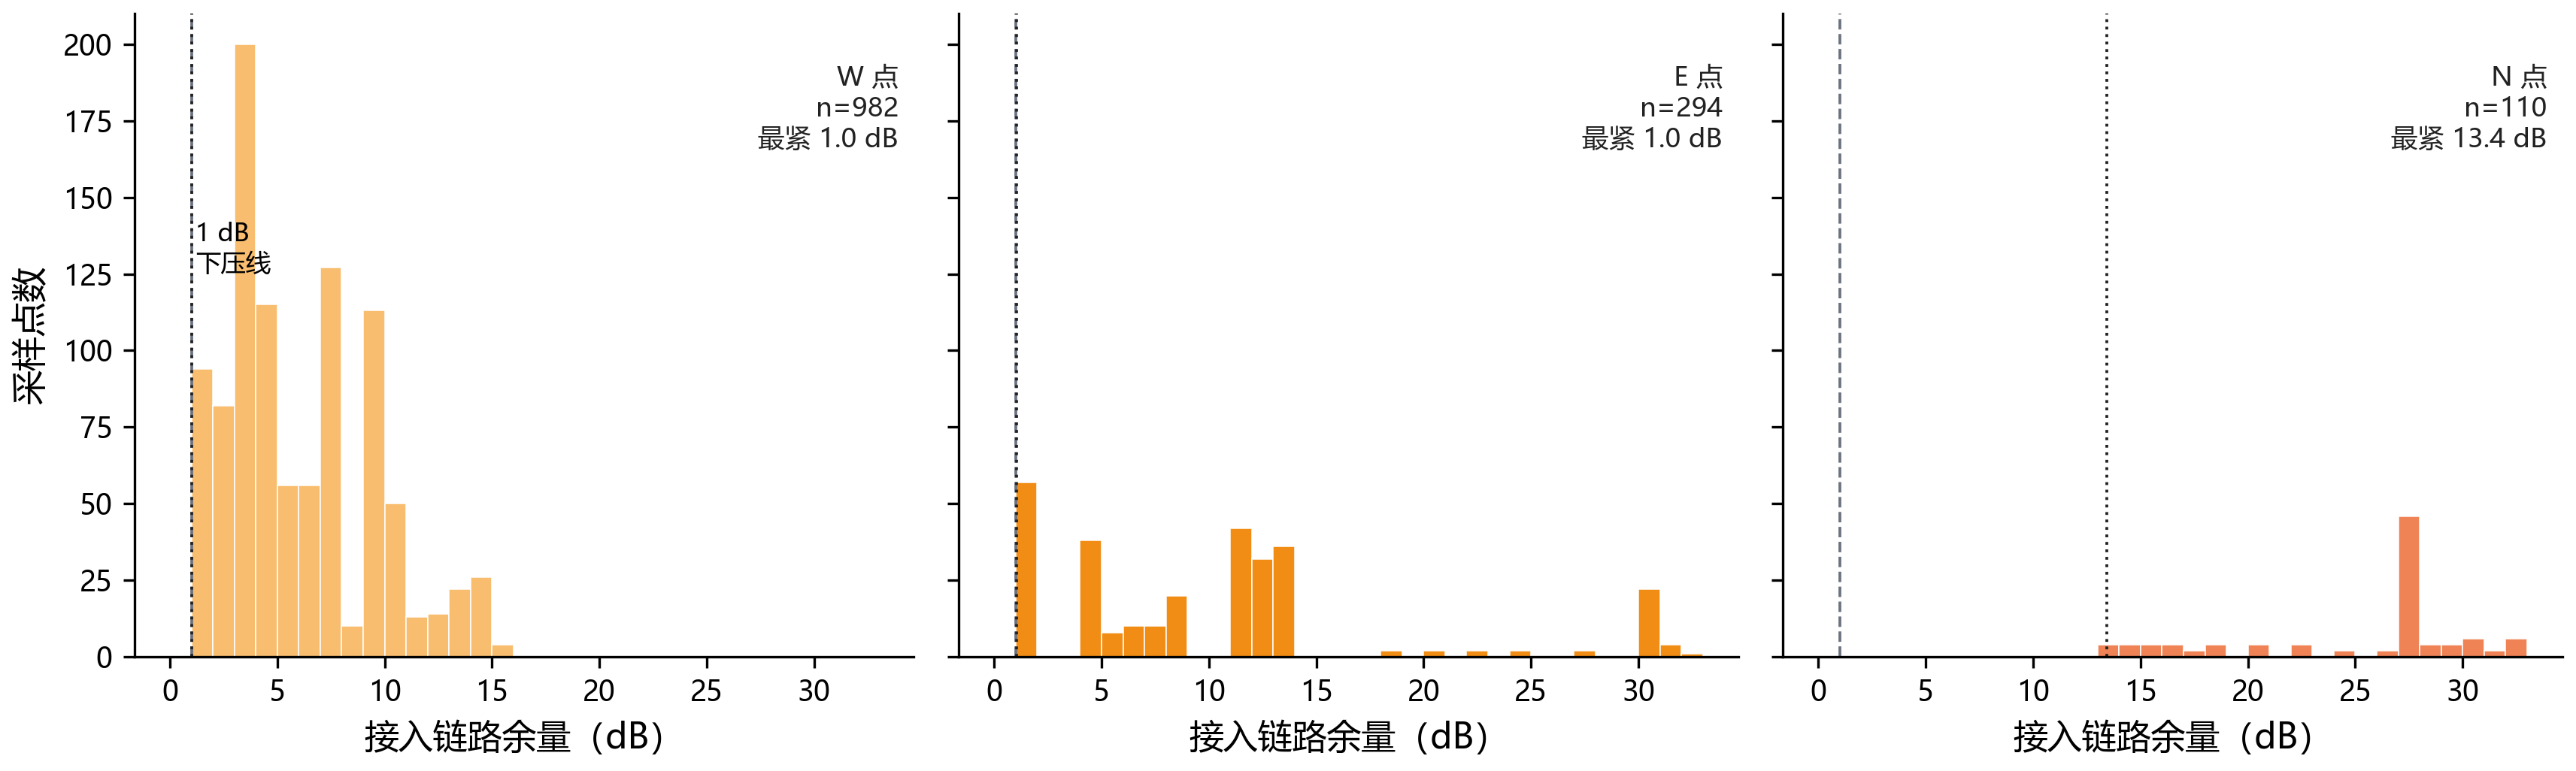
\includegraphics[width=0.98\textwidth]{figures/p3_margin_hist.png}
\caption{三个布设点接入链路余量分布（虚线为 1 dB 下压线）}
\label{fig:marginhist}
\end{figure}

\begin{table}[htbp]
\centering
\caption{各布设点接入链路余量统计（全部需中继采样点）}
\label{tab:margin}
\begin{tabular}{lcccc}
\toprule
布设点 & 覆盖采样数 & 最紧余量(dB) & 平均余量(dB) & 保障任务段数 \\
\midrule
西点 & 1096 & 0.5 & 6.2 & 33 \\
东点 & 484 & 1.0 & 13.5 & 11 \\
北点 & 211 & 13.4 & 26.0 & 4 \\
\bottomrule
\end{tabular}
\end{table}

\subsection{小结}

四类敏感性分析表明：安全余量扫描复现安全与效率的权衡且存在机型结构切换；
权重扫描确认均衡解在多目标意义下稳健；中继能源预算在 10\% 功率扰动下方案
结构不变；通信余量下压 1\,dB 时仅西点 4 个采样点接近门限，可小幅移位解决。
整体结论对参数摄动不敏感，模型可用于实际应急决策。